\section{Your Task}

As stated previously, your task for this assignment is to write a shell script,
or more specifically, a \Bash{} script. You will use this script to
produce plots of a provided \C{} program. The provided program can be
found in the resources repository.

\begin{figure}[bth]
  \centering
  % GNUPLOT: LaTeX picture with Postscript
\begingroup
  \makeatletter
  \providecommand\color[2][]{%
    \GenericError{(gnuplot) \space\space\space\@spaces}{%
      Package color not loaded in conjunction with
      terminal option `colourtext'%
    }{See the gnuplot documentation for explanation.%
    }{Either use 'blacktext' in gnuplot or load the package
      color.sty in LaTeX.}%
    \renewcommand\color[2][]{}%
  }%
  \providecommand\includegraphics[2][]{%
    \GenericError{(gnuplot) \space\space\space\@spaces}{%
      Package graphicx or graphics not loaded%
    }{See the gnuplot documentation for explanation.%
    }{The gnuplot epslatex terminal needs graphicx.sty or graphics.sty.}%
    \renewcommand\includegraphics[2][]{}%
  }%
  \providecommand\rotatebox[2]{#2}%
  \@ifundefined{ifGPcolor}{%
    \newif\ifGPcolor
    \GPcolorfalse
  }{}%
  \@ifundefined{ifGPblacktext}{%
    \newif\ifGPblacktext
    \GPblacktexttrue
  }{}%
  % define a \g@addto@macro without @ in the name:
  \let\gplgaddtomacro\g@addto@macro
  % define empty templates for all commands taking text:
  \gdef\gplbacktext{}%
  \gdef\gplfronttext{}%
  \makeatother
  \ifGPblacktext
    % no textcolor at all
    \def\colorrgb#1{}%
    \def\colorgray#1{}%
  \else
    % gray or color?
    \ifGPcolor
      \def\colorrgb#1{\color[rgb]{#1}}%
      \def\colorgray#1{\color[gray]{#1}}%
      \expandafter\def\csname LTw\endcsname{\color{white}}%
      \expandafter\def\csname LTb\endcsname{\color{black}}%
      \expandafter\def\csname LTa\endcsname{\color{black}}%
      \expandafter\def\csname LT0\endcsname{\color[rgb]{1,0,0}}%
      \expandafter\def\csname LT1\endcsname{\color[rgb]{0,1,0}}%
      \expandafter\def\csname LT2\endcsname{\color[rgb]{0,0,1}}%
      \expandafter\def\csname LT3\endcsname{\color[rgb]{1,0,1}}%
      \expandafter\def\csname LT4\endcsname{\color[rgb]{0,1,1}}%
      \expandafter\def\csname LT5\endcsname{\color[rgb]{1,1,0}}%
      \expandafter\def\csname LT6\endcsname{\color[rgb]{0,0,0}}%
      \expandafter\def\csname LT7\endcsname{\color[rgb]{1,0.3,0}}%
      \expandafter\def\csname LT8\endcsname{\color[rgb]{0.5,0.5,0.5}}%
    \else
      % gray
      \def\colorrgb#1{\color{black}}%
      \def\colorgray#1{\color[gray]{#1}}%
      \expandafter\def\csname LTw\endcsname{\color{white}}%
      \expandafter\def\csname LTb\endcsname{\color{black}}%
      \expandafter\def\csname LTa\endcsname{\color{black}}%
      \expandafter\def\csname LT0\endcsname{\color{black}}%
      \expandafter\def\csname LT1\endcsname{\color{black}}%
      \expandafter\def\csname LT2\endcsname{\color{black}}%
      \expandafter\def\csname LT3\endcsname{\color{black}}%
      \expandafter\def\csname LT4\endcsname{\color{black}}%
      \expandafter\def\csname LT5\endcsname{\color{black}}%
      \expandafter\def\csname LT6\endcsname{\color{black}}%
      \expandafter\def\csname LT7\endcsname{\color{black}}%
      \expandafter\def\csname LT8\endcsname{\color{black}}%
    \fi
  \fi
    \setlength{\unitlength}{0.0500bp}%
    \ifx\gptboxheight\undefined%
      \newlength{\gptboxheight}%
      \newlength{\gptboxwidth}%
      \newsavebox{\gptboxtext}%
    \fi%
    \setlength{\fboxrule}{0.5pt}%
    \setlength{\fboxsep}{1pt}%
    \definecolor{tbcol}{rgb}{1,1,1}%
\begin{picture}(7200.00,5040.00)%
    \gplgaddtomacro\gplbacktext{%
      \csname LTb\endcsname%%
      \put(1443,440){\makebox(0,0)[r]{\strut{}$0$}}%
      \put(1443,1316){\makebox(0,0)[r]{\strut{}$0.2$}}%
      \put(1443,2192){\makebox(0,0)[r]{\strut{}$0.4$}}%
      \put(1443,3067){\makebox(0,0)[r]{\strut{}$0.6$}}%
      \put(1443,3943){\makebox(0,0)[r]{\strut{}$0.8$}}%
      \put(1443,4819){\makebox(0,0)[r]{\strut{}$1$}}%
      \put(1575,220){\makebox(0,0){\strut{}$0$}}%
      \put(2451,220){\makebox(0,0){\strut{}$0.2$}}%
      \put(3327,220){\makebox(0,0){\strut{}$0.4$}}%
      \put(4202,220){\makebox(0,0){\strut{}$0.6$}}%
      \put(5078,220){\makebox(0,0){\strut{}$0.8$}}%
      \put(5954,220){\makebox(0,0){\strut{}$1$}}%
    }%
    \gplgaddtomacro\gplfronttext{%
    }%
    \gplbacktext
    \put(0,0){
\includegraphics[width={360.00bp},height={252.00bp}]{figures/monte_carlo_grid}}%
    \gplfronttext
  \end{picture}%
\endgroup

  \caption{\label{figure:monte_carlo_grid}
    Blue points have distance less than or equal to 1, and hence belong both in the square and the circle, red points are a part of the square but not the circle.
  }
\end{figure}


All the program does is print the Monte Carlo estimation for $\pi$ after each random point it tests. For those unacquainted with Monte Carlo estimation of $\pi$, we use a large number of points
in a square with an inscribed quadrant. The ratio of the number of points in the quadrant to the number of points in the square is the ratio of the to areas:
\begin{itemize}
  \item Area of Square with side $l$ is $l^2$
  \item Area of a quadrant of a circle with radius $l$ is $\frac{\pi l^2}{4}$
  \item The ratio of these areas is $\frac{\pi}{4}$
\end{itemize}
The process is as follows: We will uniformly scatter a number of points in a square, and measure the number of points that fall within the quadrant (distance from origin less than or equal to 1) and the other points. The C program will output the estimated value of $\pi$ after every point for $n$ number of points. We have provided an example of this scatter in Figure~\ref*{figure:monte_carlo_grid}.

Using the provided Monte Carlo program, you are expected to:
\begin{enumerate}
  \item Familiarize yourself with the syntax of \C{}.
  \item Understand what the provided program is doing. You will want to attend
    section for any parts you are unsure about.
  \item Produce interesting plots using the Monte Carlo estimations produced by the
    provided program. You should use \texttt{gnuplot} to produce these plots,
    and everything should be automated by means of a \Bash{} script.
\end{enumerate}


\begin{shlisting}{Output for the monte\_carlo program}
$ ./monte_carlo -n 10
 Iteration       Pi                x                y circle
         0        4         0.445822          0.55245      1
         1        4         0.772659         0.506885      1
         2  2.66667         0.999439        0.0812311      0
         3        3         0.727855         0.515805      1
         4      3.2         0.199699         0.390919      1
         5  3.33333         0.579692         0.536917      1
         6  3.42857         0.358613         0.367796      1
         7      3.5         0.241639         0.905172      1
         8  3.55556         0.974999        0.0754683      1
         9      3.2         0.862372         0.706275      0
\end{shlisting}

Here is an example output for the provided program up to 10 points.
The output provides you with the point number, the estimated value
of $\pi$ at the current point, its $x$ and $y$ coordinates, as well
as a 1 or 0 value indicating if it is in the circle, where 1 means
it is inside the circle.

Refer to Figures  \ref{figure:monte_carlo_grid}, \ref{figure:monte_carlo}
for the example plot that were created using the provided program.
Now that you know your task, we will now give a brief overview on
\Bash{} scripting.

\begin{figure}[htb]
  \centering
  % GNUPLOT: LaTeX picture with Postscript
\begingroup
  \makeatletter
  \providecommand\color[2][]{%
    \GenericError{(gnuplot) \space\space\space\@spaces}{%
      Package color not loaded in conjunction with
      terminal option `colourtext'%
    }{See the gnuplot documentation for explanation.%
    }{Either use 'blacktext' in gnuplot or load the package
      color.sty in LaTeX.}%
    \renewcommand\color[2][]{}%
  }%
  \providecommand\includegraphics[2][]{%
    \GenericError{(gnuplot) \space\space\space\@spaces}{%
      Package graphicx or graphics not loaded%
    }{See the gnuplot documentation for explanation.%
    }{The gnuplot epslatex terminal needs graphicx.sty or graphics.sty.}%
    \renewcommand\includegraphics[2][]{}%
  }%
  \providecommand\rotatebox[2]{#2}%
  \@ifundefined{ifGPcolor}{%
    \newif\ifGPcolor
    \GPcolorfalse
  }{}%
  \@ifundefined{ifGPblacktext}{%
    \newif\ifGPblacktext
    \GPblacktexttrue
  }{}%
  % define a \g@addto@macro without @ in the name:
  \let\gplgaddtomacro\g@addto@macro
  % define empty templates for all commands taking text:
  \gdef\gplbacktext{}%
  \gdef\gplfronttext{}%
  \makeatother
  \ifGPblacktext
    % no textcolor at all
    \def\colorrgb#1{}%
    \def\colorgray#1{}%
  \else
    % gray or color?
    \ifGPcolor
      \def\colorrgb#1{\color[rgb]{#1}}%
      \def\colorgray#1{\color[gray]{#1}}%
      \expandafter\def\csname LTw\endcsname{\color{white}}%
      \expandafter\def\csname LTb\endcsname{\color{black}}%
      \expandafter\def\csname LTa\endcsname{\color{black}}%
      \expandafter\def\csname LT0\endcsname{\color[rgb]{1,0,0}}%
      \expandafter\def\csname LT1\endcsname{\color[rgb]{0,1,0}}%
      \expandafter\def\csname LT2\endcsname{\color[rgb]{0,0,1}}%
      \expandafter\def\csname LT3\endcsname{\color[rgb]{1,0,1}}%
      \expandafter\def\csname LT4\endcsname{\color[rgb]{0,1,1}}%
      \expandafter\def\csname LT5\endcsname{\color[rgb]{1,1,0}}%
      \expandafter\def\csname LT6\endcsname{\color[rgb]{0,0,0}}%
      \expandafter\def\csname LT7\endcsname{\color[rgb]{1,0.3,0}}%
      \expandafter\def\csname LT8\endcsname{\color[rgb]{0.5,0.5,0.5}}%
    \else
      % gray
      \def\colorrgb#1{\color{black}}%
      \def\colorgray#1{\color[gray]{#1}}%
      \expandafter\def\csname LTw\endcsname{\color{white}}%
      \expandafter\def\csname LTb\endcsname{\color{black}}%
      \expandafter\def\csname LTa\endcsname{\color{black}}%
      \expandafter\def\csname LT0\endcsname{\color{black}}%
      \expandafter\def\csname LT1\endcsname{\color{black}}%
      \expandafter\def\csname LT2\endcsname{\color{black}}%
      \expandafter\def\csname LT3\endcsname{\color{black}}%
      \expandafter\def\csname LT4\endcsname{\color{black}}%
      \expandafter\def\csname LT5\endcsname{\color{black}}%
      \expandafter\def\csname LT6\endcsname{\color{black}}%
      \expandafter\def\csname LT7\endcsname{\color{black}}%
      \expandafter\def\csname LT8\endcsname{\color{black}}%
    \fi
  \fi
    \setlength{\unitlength}{0.0500bp}%
    \ifx\gptboxheight\undefined%
      \newlength{\gptboxheight}%
      \newlength{\gptboxwidth}%
      \newsavebox{\gptboxtext}%
    \fi%
    \setlength{\fboxrule}{0.5pt}%
    \setlength{\fboxsep}{1pt}%
    \definecolor{tbcol}{rgb}{1,1,1}%
\begin{picture}(7200.00,5040.00)%
    \gplgaddtomacro\gplbacktext{%
      \csname LTb\endcsname%%
      \put(946,440){\makebox(0,0)[r]{\strut{}$-1$}}%
      \csname LTb\endcsname%%
      \put(946,1425){\makebox(0,0)[r]{\strut{}$-0.5$}}%
      \csname LTb\endcsname%%
      \put(946,2410){\makebox(0,0)[r]{\strut{}$0$}}%
      \csname LTb\endcsname%%
      \put(946,3394){\makebox(0,0)[r]{\strut{}$0.5$}}%
      \csname LTb\endcsname%%
      \put(946,4379){\makebox(0,0)[r]{\strut{}$1$}}%
      \csname LTb\endcsname%%
      \put(1078,220){\makebox(0,0){\strut{}$1$}}%
      \csname LTb\endcsname%%
      \put(1812,220){\makebox(0,0){\strut{}$4$}}%
      \csname LTb\endcsname%%
      \put(2545,220){\makebox(0,0){\strut{}$16$}}%
      \csname LTb\endcsname%%
      \put(3279,220){\makebox(0,0){\strut{}$64$}}%
      \csname LTb\endcsname%%
      \put(4012,220){\makebox(0,0){\strut{}$256$}}%
      \csname LTb\endcsname%%
      \put(4746,220){\makebox(0,0){\strut{}$1024$}}%
      \csname LTb\endcsname%%
      \put(5479,220){\makebox(0,0){\strut{}$4096$}}%
      \csname LTb\endcsname%%
      \put(6213,220){\makebox(0,0){\strut{}$16384$}}%
    }%
    \gplgaddtomacro\gplfronttext{%
      \csname LTb\endcsname%%
      \put(209,2409){\rotatebox{-270}{\makebox(0,0){\strut{}Error}}}%
      \csname LTb\endcsname%%
      \put(3940,4709){\makebox(0,0){\strut{}Monte Carlo Error Estimation}}%
    }%
    \gplbacktext
    \put(0,0){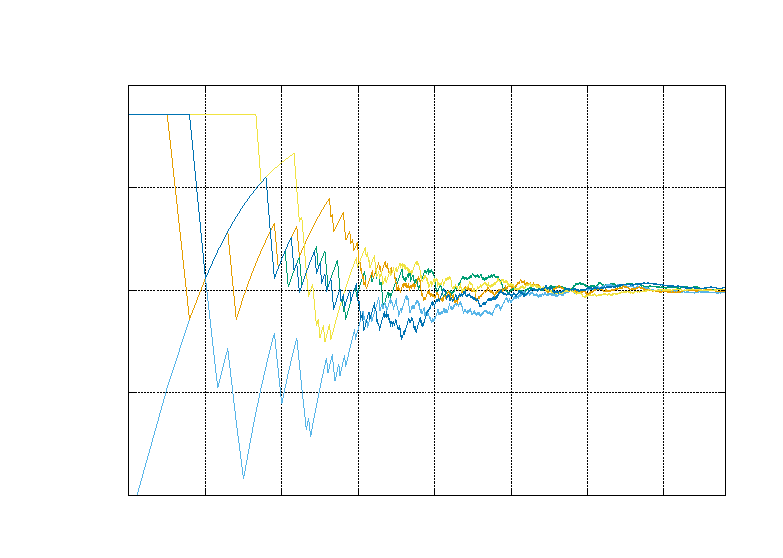
\includegraphics[width={360.00bp},height={252.00bp}]{figures/monte_carlo}}%
    \gplfronttext
  \end{picture}%
\endgroup

  \caption{\label{figure:monte_carlo}
    The value of the difference between the estimated $\pi$ and
    $pi$ gets closer to zero as we increase iterations. The different
    colors represent different seeds for the random number generator.}
\end{figure}
